\documentclass{article}
\usepackage{amsmath}
\usepackage{amssymb}
\usepackage{graphicx}
\title{Response To Reviews - A Data-Driven Framework for Neural Field Modeling}
\author{D. Freestone, P. Aram, M. Dewar, K. Scerri, D. Grayden, V. Kadirkamanathan}

\begin{document}
    \maketitle
    
    \section{Reviewer 1}
    
        We first adress the reviewer's main concerns, followed by the reviewer's additional comments.
        
    \subsection{Main Concerns}
    
    \begin{enumerate}
        \item Do not use real data for the validation of their approach
        \item Assume that a few kernel basis functions accurately represent the actual connectivity kernel, which might not be the case when using real data;
        \item Do not consider the EEG/MEG lead field when constructing their mapping between the membrane voltage and the electrophysiological data (observation function)
    \end{enumerate}
    
    \subsection{Additional Comments}
    
    \begin{enumerate}
        \item The discrepancy of the results in Experiment II where the weights of the basis functions are not in agreement with the actual parameters while the recontructed kernels seem satisfying.
        \item The use of Euler discretisation and how this affects the system's behavior.
        \item The derivation of Equations (30) and (31) [spacing and width of basis functions] and make them more transparent for the general audience.
        \item The existing literature on inversion schemes for similar models of brain activity.
        \item In section 3, Table 6 is mentioned however there is no such table in the ms.
    \end{enumerate}
    
    \section{Reviewer 2}
    
    We thank the author for their encouraging review. Each point raised is dealt with in turn.

\begin{enumerate}
    \item The handling of the (to borrow a term from numerical weather forecasting) `sub-grid scale physics' is inadequate for nervous systems (see, e.g., equation 8 [The nonlinear IntegroDifference Equation]). I do very much appreciate the spectral estimation of spatial and temporal scales. But the model errors are lumped into an iid model error term that is not realistic. For instance, the flow of potassium in the extracellular spaces has a known dynamic that will affect network excitability, generating important sub-grid dynamics that is anything but iid. See, for instance, the example in Ullah et al PLoS Comp Biol 2010 where without such dynamics, state tracking and parameter estimation for a neural system fails. A beautiful overview of sub-grid effects in data assimilation is found in Kalnay's 2003 book. I would very much value the authors comments on these issues. I guess were I to respond to this question, that I might consider extending the model error term to an autoregressive model. But I will let the authors answer this question.\\
    \emph{talk about model order}
\item Although we all know the 1970s version of Wilson and Cowan's field equations, there was an intriguing stochasticization of these equations by Benayoun et al PloS Comp Biol 2010. I and others will value the authors' thoughts of how a more palatable stochasticization of these field equations might influence the future development of the data-assimilation framework presented in this paper.
\item This is NeuroImage, not the Physical Review. Although most of this framework involves mathematics that is reasonable to follow for typical readers of this journal, I would suggest that the authors explain and expand a bit on the introduction of Green's functions where introduced in equation 6.
\item What is the relation of the substitution of the temporal and spatial basis functions as employed in this paper to Galerkin's projection? How do the two techniques differ? If this is close, the non-local case for a Galerkin projection (typically used in diffusive processes) has not, to my knowledge, been done. Certainly not in a way that is obvious for neural field theory. Perhaps this is my ignorance. This seems important to clarify for the rest of us.
\item In the isotropic and translationally invariant case examined here, would a Fourier basis for temporal and spatial structure have been a formally correct alternative?\\
\emph{Gaussians has semi-compact support but Fourier basis functions are global functions. Gaussian can be easily extended to higher dimension (dont know about the Fourier basis functions), any orthonormal basis functions like Fourier basis functions simplify our equations, $\Gamma$ becomes identity matrix, but using Gaussian basis functions equations are in their generic form.}
\item In equation 29, what would a reasonable $v_c$ be for a real neuronal system (mammalian) given the number of neurons and scale of electrodes? I am concerned that it might be much higher than any of us wish to consider. One would perhaps be saved by the filter characteristics of brain (e.g. Phys. Rev. E 73, 051911 (2006)).
\item The two covariance inflation parameters in equation 41 make me cringe. How are we best to adjust these fudge factors?
\emph{The positive constant $\alpha$ determines the spread of the sigma points around $\mathbf{\bar x}$ which can be made arbitrary small (e.g. $0<\alpha\le 10^{-4} $) to minimise higher order effect (cite Julier (The Scaled Unscented Transformation) and  Haykin (Kalman filtering and neural network) , and  $\kappa$ is an additional scaling parameter which is usually set to $3-n_x$. cite Julier A New Approach for Filtering Nonlinear Systems}



\item I understand that the Mexican Hat bases are in this paper often a composite of $\theta_0$, $\theta_1$, and $\theta_2$, representing short range excitation, short range inhibition, and long range excitation. But many will be confused by this subtlety, and at times in the text the Mexican Hat basis is described as if it were a single function. I would show how the theta's sum to create the general spatial basis shape of the hat in figure 1, and go through the paper in order to clarify this issue.\\
\emph{I think we need to show each kernel basis function in Figure 1}
 \begin{figure*}[!ht]
 \begin{center}
 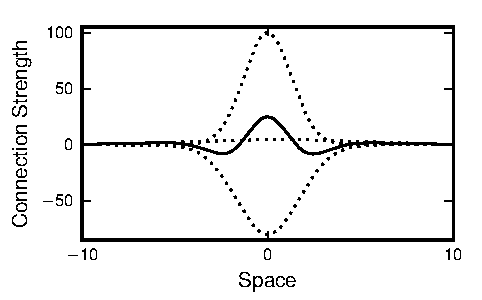
\includegraphics{/Graph/pdf/fig1_revised.pdf} 
 \end{center}
 \caption{}
 \label{fig:Figure1}
 \end{figure*}

\item A few comments on how to adapt the smoother for real time implementation would be helpful. I presume that one would perform the smoothing during a training phase. But one would also wish to adapt in real time as observation or control scenarios progressed. A few words of perspective would be invaluable to help others translate the author's wisdom on this method to other applications.
\item Figure 4. Should the axes be indicated as spatial frequency rather than just Hz?
\item Page 45, Appendix D, Par 1, line 6: should `transform of a n-' should be `transform of an n-' ? I am grammatically challenged perhaps.
\end{enumerate}

\end{document}